\documentclass[a4paper,12pt,titlepage]{article}

%Εισαγωγή γλωσσικής υποστήριξης
%ελληνικό hyphenation

\usepackage{fontspec}
\usepackage{xunicode}
\usepackage{xltxtra}
\usepackage{xgreek}
\usepackage[colorlinks]{hyperref}
\usepackage{enumerate}
\usepackage{amsmath}
%\usepackage{tikz}
%η γραμματοσειρά
%\setmainfont[Mapping=tex-text]{Times New Roman} %απλοποιημένο σε σχέση με το άρθρο
\setmainfont[Mapping=tex-text]{Linux Libertine} 
%page orientation
\usepackage{a4wide}
\voffset = -0.5in
\textheight = 664pt

%Άλλα χρήσιμα πακέτα
\usepackage{graphicx} 	%εισαγωγή εικόνων jpg/png κλπ
\usepackage{listings}
\lstset{commentstyle=\textit,
captionpos=b,
breakatwhitespace=true,
showstringspaces=false,
breaklines=true,
keywordstyle=\color{black}\bfseries,
float=htb,
frame=single}

%απενεργοποίηση του indent στις νέες παραγράφους
\parindent=0in

%macro που δίνει το μέγιστο επιτρεπτό μέγεθος σε μια εικόνα χωρίς να παραβιάζει τα όρια του LaTeX
\makeatletter
\def\maxwidth{
\ifdim\Gin@nat@width>\linewidth
\linewidth
\else
\Gin@nat@width
\fi
}

\makeatother

\title{1η Άσκηση\\kn}
\author{AxiP}
\date{\today}

\begin{document}

\pagestyle{headings}    %αρίθμηση στο πάνω μέρος της σελίδας

%\maketitle
\begin{titlepage}
\begin{center}

\includegraphics[width=50mm]{pyrforos.pdf}\\[0.5cm]
\textbf{\LARGE ΕΘΝΙΚΟ ΜΕΤΣΟΒΙΟ ΠΟΛΥΤΕΧΝΕΙΟ}\\
\textrm{\Large Σχολή Εφαρμοσμένων Μαθηματικών και Φυσικών Επιστημών}\\[2.0cm]
\Huge{Τεχνολογία των laser\\}
\Large{\textit{6o εξάμηνο, ΣΕΜΦΕ}}\\[2.0cm]
\Large{\textit{\textbf{Κατασκευή τροφοδοτικού διοδικού laser}}}\\[5.0cm]
\normalsize

\begin{minipage}{0.49\textwidth}
\begin{flushleft}
\textbf{Αχιλλέας Πιπινέλλης}, 09103163
\end{flushleft}
\end{minipage}
\begin{minipage}{0.49\textwidth}
\begin{flushright}
\textbf{\\
\textit{Η/Μ Παράδοσης:} 2 Ιουνίου 2012}
\end{flushright}
\end{minipage}

%\maketitle

\vfill
%bottom of the page
{Αθήνα, 2012}

\end{center}
\end{titlepage}

\section{Σκοπός του πειράματος}

Στην παρούσα άσκηση θα εξετάσουμε πως δουλεύει ένα διοδικό laser και θα μελετήσουμε τη σταθεροποίηση του ρεύματος, εργαζόμενοι πάνω σε ένα breadborad του οποίου τα εξαρτήματα θα απαριθμήσουμε παρακάτω.

\section{Θεωρία}

\subsection{Διοδικό Laser}
Το διοδικό laser είναι η ένωση ενός ημιαγωγού τύπου $P$ με έναν τύπου $N$. Οι ημιαγωγοί είναι υλικά που αποτελούνται από στοιχεία της τέταρτης ομάδας (IV) του περιοδικού πίνακα και έχουν ηλεκτρικές ιδιότητες που βρίσκονται κάπου ανάμεσα σε αυτές των αγωγών και αυτές των μονωτών. \\\\
H τεχνολογία των ημιαγωγών σπάνια χρησιμοποιεί καθαρούς ημιαγωγούς. Για να ελεγχθεί ο αριθμός φορέων φορτίου σε έναν ημιαγωγό, συνήθως χρησιμοποιείται η διαδικασία της πρόσμιξης (doping) του καθαρού ημιαγωγού με κάποιο άλλο χημικό στοιχείο. Το ποσό των ξένων στοιχείων ελέγχεται, και μπορεί να είναι δύο τύπων. Αν το υλικό νόθευσης είναι στοιχείο που ανήκει στην ομάδα $V$ του περιοδικού πίνακα, καλείται δότης (donor). Αν ανήκει στην ομάδα III τότε ονομάζεται δέκτης (acceptor). Οι νοθευμένοι ημιαγωγοί με δότες ηλεκτρονίων καλούνται ημιαγωγοί τύπου-n (n-type semiconductors), ενώ αυτοί που είναι νοθευμένοι με δέκτες ηλεκτρονίων ονομάζονται ημιαγωγοί τύπου-p (p-type semiconductors). Στους ημιαγωγούς τύπου-n, τα ηλεκτρόνια είναι φορείς πλειονότητας(majority carriers) και οι οπές φορείς μειονότητας(minority coarriers). Σε έναν ημιαγωγό τύπου-p οι φορείς πλειονότητας και μειονότητας αντιστρέφονται.\\\\
Ένας ενδογενής ημιαγωγός δεν έχει ιδιότητες που να τον καθιστούν χρήσιμο στην κατασκευή ηλεκτρονικών κυκλωμάτων. Όταν όμως ένα κομμάτι ημιαγωγού τύπου-p και ένα τύπου-n έρθουν σε επαφή, σχηματίζουν μία pn επαφή (pn junction), η οποία έχει διάφορες ενδιαφέρουσες ιδιότητες. Για να λειτουργήσει το laser πρέπει να υπάρχει μια περιοχή $PN$ που συνυπάρχουν ηλεκτρόνια και οπές. Για να επιτευχθεί οπτική εκπομπή πρέπει η περιοχή $PN$ να είναι ορθά πολωμένη και να άγει. Η συχνότητα της εκπεμπόμενης ακτινοβολίας αντιστοιχεί στη διαφορά ενέργειας μεταξύ των σταθμών που καταλαμβάνει το ηλεκτρόνιο στη ζώνη αγωγιμότητας και της οπής στη ζώνη σθένους. \\\\
Για να λειτουργήσει η παραπάνω διάταξη σαν laser απαιτείται εξαναγκασμένη εκπομπή που επιτυγχάνεται με την αντιστροφή πληθυσμού, δηλαδή το πλήθος των ηλεκτρονίων στη ζώνη αγωγιμότητας να είναι μεγαλύτερο από το πλήθος των οπών στη ζώνη σθένους. Διαφορετικά λειτουργεί σαν απλό LED. Για να ξεκινήσει η εκπομπή laser απαιτείται το ρεύμα να υπερβεί μια κρίσιμη τιμή, το ρεύμα κατωφλίου, η οποία εξαρτάται από τη θερμοκρασία της διόδου.

\newpage
\subsection{Τελεστικός ενισχυτής}
Σε μερικές εφαρμογές των laser η φωτεινότητα της δέσμης πρέπει να είναι απόλυτα ελεγχόμενη. Για παράδειγμα στην οπτική μετάδοση σήματος το σήμα δίνεται συναρτήσει της φωτεινότητας, οπότε μια μικρή μεταβολή της έντασης της ακτινοβολίας θα έδινε λάθος σήμα. Άρα θέλουμε σταθερή φωτεινότητα, δηλαδή σταθερό ρεύμα. Αυτό επιτυγχάνεται με ένα κύκλωμα τελεστικού ενισχυτή, με κύριο συστατικό του το τρανζίστορ.

Ο τελεστικός ενισχυτής έχει δύο εισόδους. Η μία είναι μη αναστρέφουσα (+), δηλαδή είναι σε φάση με την έξοδο και η άλλη αναστρέφουσα (-), δηλαδή είναι σε διαφορά φάσης $\pi$ με την έξοδο. Η λειτουργία του είναι να κρατάει τις δύο τάσεις εισόδου ίσες, κάτι που προκαλεί μεγάλη ενίσχυση στην έξοδο. Έτσι, με μία μικρή μεταβολή στην είσοδο της τάξης των $mV$, προκαλεί στην έξοδο τάση μερικών $Volts$.

\subsection{Τρανζίστορ}
Το τρανζίστορ είναι κρύσταλλος ημιαγώγιμου υλικού (συνήθως πυρίτιο) με τρεις εμπλουτισμένες περιοχές $NPN$ ή $PNP$. Οι τρεις περιοχές τού τρανζίστορ ονομάζονται εκπομπός, βάση και συλλέκτης. Ο ένας ακροδέκτης είναι κοινός και σχηματίζει δύο βρόγχους με τους άλλους δύο ακροδέκτες. Στην άσκηση χρησιμοποιούμε κύκλωμα κοινής βάσης, όπου υπάρχει ροή μικρού ρεύματος από τον εκπομπό στη βάση και μεγαλύτερου ρεύματος από τον εκπομπό στο συλλέκτη.
Στο κύκλωμα του τροφοδοτικού του laser απαιτούμε σταθερό ρεύμα, αλλά η τάση τροφοδοσίας είναι μεταβαλλόμενη. Άρα χρειαζόμαστε μεταβλητή αντίσταση, ώστε να παραμένει το ρεύμα σταθερό. Η μεταβολή της αντίστασης όμως θέλουμε να γίνεται σε πραγματικό χρόνο και με δεδομένο τις πολύ γρήγορες μεταβολές της τάσης, απαιτείται ηλεκτρονικός ροοστάτης. Τον ρόλο του ροοστάτη τον παίζει το τρανζίστορ, το οποίο μεταβάλει την αγωγιμότητά του, ώστε και οι δύο βρόγχοι του να διαρρέονται από την ίδια τιμή ρεύματος.

\newpage

\section{Μέθοδος}

Η πηγή $E_{B}$ δίνει ρεύμα στη δίοδο laser, όπως φαίνεται στο Σχήμα 1 (κλάδος Β). Επειδή το ρεύμα αυτό πρέπει να παραμένει σταθερό, χρησιμοποιείται ένας τελεστικός ενισχυτής όπως φαίνεται στο Σχήμα 1 (κλάδος Α). Εϊναι πιθανό η πηγή $E_{B}$ να εμφανίζει μερικές ανεπιθύμητες μεταβολές, οι οποίες θα εμφανίζονται και στα άκρα της αντίστασης $R_{3}$. H τάση αυτή $V_{2}$ στα άκρα της $R_{3}$ οδηγείται στην αναστρέφουσα είσοδο του τελεστικού ενισχυτή. Στη μη αναστρέφουσα είσοδο εμφαρμόζεται μία σταθερή τάση $V_{1}$. Ο ρόλος του τελεστικού ενισχυτή είναι να διατηρεί τις τάσεις $V_{1}$ και $V_{2}$ συνχεχώς ίσες. Έτσι θα παράγει μία τάση στην έξοδό του, τέτοια ώστε να μεταβάλλεται η αγωγιμότητα του ημιαγωγού $Τ$, ώστε να εξουδετερώνονται οι ανεπιθύμητες μεταβολές του ρεύματος $Ι$.

\begin{figure}[!h]
\centering
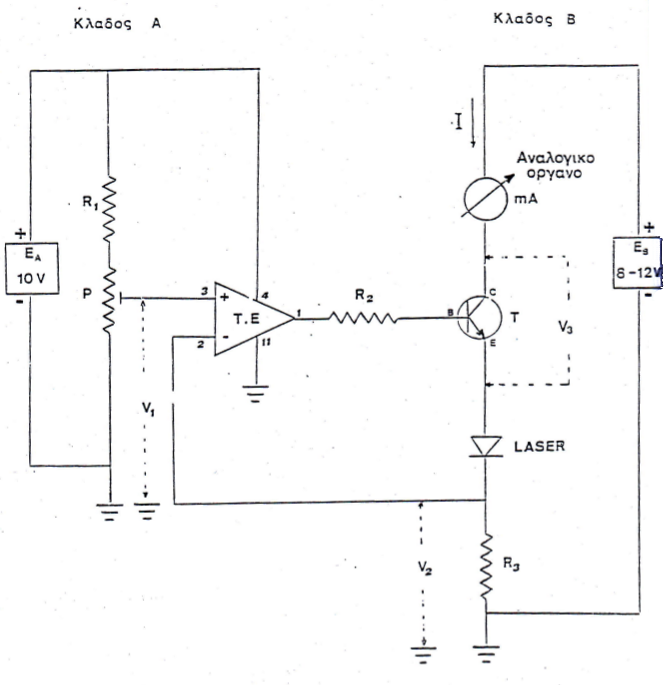
\includegraphics[width=\maxwidth]{diataksi.png}\\[0.3cm]
\caption{Η πειραματική διάταξη}
\end{figure}

\subsection{Πειραματική Διάταξη}

Η άσκηση θα εκτελεστεί σε  πλακέτα γενικών κατασκευών (breadborad). H διάταξη του πειράματος περιλαμβάνει τα εξής εξαρτήματα:

\begin{itemize}
  \item Δύο τροφοδοτικά χαμηλής τάσεως($E_{A}=10V$, $E_{B}=15V$) τα οποία τροφοδοτούν τους κλάδους Α και Β αντίστοιχα (βλ. Σχήμα 1).
  \item Αναλογικό όργανο για τη μέτρηση του ρεύματος $Ι$ του laser.
  \item Ψηφιακό όργανο για τη μέτρηση των τάσεων $V_{1}$, $V_{2}$, $V_{3}$.
  \item Μία δίοδο laser.
  \item Ένα ολοκληρωμένο κύκλωμα.
  \item	Έναν ημιαγωγό.
  \item Τρεις αντιστάσεις $R_{1}$, $R_{2}$, $R_{3}$.
  \item	Ένα ποτενσιόμετρο.
  \item	Μία πλακέτα (breadboard).
\end{itemize}

\newpage

\section{Εκτέλεση}

Ρυθμίσαμε την τάση $E_{B}=10\pm{0.1}V$ και μεταβάλαμε την τάση $V_{1}$ με το ποτενσιόμετρο από $0V-4.5V$ με βήμα $0.5V$. Τα αποτελέσματα παρουσιάζονται στον πίνακα 1.

\begin{table}[h!]
\begin{center}
    \begin{tabular}{ | c | c |}
    \hline
     $V_{1} (Volt)$ & $V_{2} (Volt)$\\ \hline
     0	  &   0\\ \hline
     0.49 & 0.49\\ \hline
     0.99 & 1.00\\ \hline
     1.51 & 1.51\\ \hline
     2.01 & 2.01\\ \hline
     2.52 & 2.52\\ \hline
     3.01 & 3.02\\ \hline
     3.49 & 3.49\\ \hline
     4.02 & 4.02\\ \hline
     4.50 & 4.50\\ \hline
    \end{tabular}
\end{center}
\caption{Τάση $V_{1}$, $V_{2}$ με $E_{B}=10V$ }
\end{table}

Παρατηρούμε πως δεν υπάρχει διαφορά τάσης, άρα ο τελεστικός ενισχυτής διατηρεί τις δύο τάσεις ίσες.

\newpage

Στη συνέχεια ρυθμίσαμε το ρεύμα μέσω του ποτενσιόμετρου να είναι $35\pm{1}mA$ και μεταβάλλοντας την τάση της πηγής $E_{B}$ από $8V-12V$ με βήμα $0.5V$ μετρήσαμε πως μεταβάλλεται το ρεύμα συναρτήσει της τάσης. Το ίδιο κάναμε και για $I=45\pm{1}mA$. Όπως παρατηρεί κανείς, το ρεύμα και στις δύο περιπτώσεις παραμένει το ίδιο. Τα αποτελέσματα παρουσιάζονται στον Πίνακα 2 και το Σχήμα 2.

\begin{table}[h!]
\begin{center}
    \begin{tabular}{ | c | c | c |}
    \hline
     $E_{B}(Volt)$ & $I_{35} (mA)$ & $I_{45} (mA)$\\ \hline
     8.0  & 35	& 45 \\ \hline
     8.5  & 35	& 45 \\ \hline
     9.0  & 35	& 45 \\ \hline
     9.5  & 35	& 45 \\ \hline
     10.0 & 35	& 45 \\ \hline
     10.5 & 35	& 45 \\ \hline
     11.0 & 35	& 45 \\ \hline
     11.5 & 35	& 45 \\ \hline
     12.0 & 35	& 45 \\ \hline
    \end{tabular}
\end{center}
\caption{Μεταβολή του ρεύματος $I$ συναρτήσει της τάσης $E_{B}$}
\end{table}

\begin{figure}[!h]
\centering
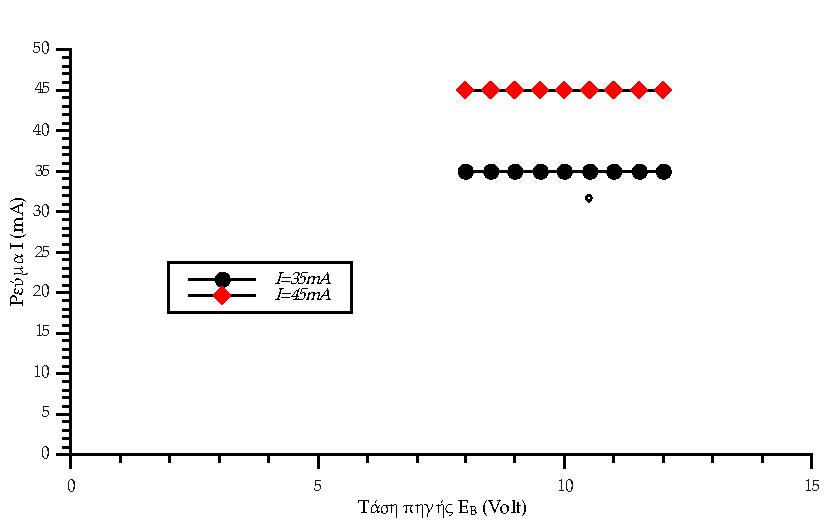
\includegraphics[width=\maxwidth]{graph1.pdf}\\[0.3cm]
\caption{Μεταβολή του ρεύματος $I$ συναρτήσει της τάσης $E_{B}$}
\end{figure}

\newpage

Ρυθμίζοντας το ρεύμα σταθερό στα $40\pm{1}mA$, μεταβάλαμε την τάση $E_{B}$ απο $8V-12V$ με βήμα $0.5$ και πήραμε μετρήσεις των τάσεων $V_{2}$ και $V_{3}$. Τα αποτελέσματα φαίνονται στον πίνακα 3.

\begin{table}[h!]
\begin{center}
    \begin{tabular}{ | c | c | c |}
    \hline
     $E_{B}(Volt)$ & $V_{2} (Volt)$ & $V_{3} (Volt)$\\ \hline
     8.0  	& 2.65	& 3.20 \\ \hline
     8.5  	& 3.04	& 3.18 \\ \hline
     9.0  	& 3.78	& 3.15 \\ \hline
     9.5  	& 4.30	& 3.15 \\ \hline
     10.0 	& 4.90	& 3.14 \\ \hline
     10.5 	& 5.71	& 3.14 \\ \hline
     11.0 	& 6.25	& 3.14 \\ \hline
     11.5 	& 6.77	& 3.14 \\ \hline
     12.0 	& 7.32	& 3.13 \\ \hline
    \end{tabular}
\end{center}
\caption{Μεταβολή των τάσεων $V_{2}$ και $V_{3}$ συναρτήσει της τάσης $E_{B}$ για $I=40mA$}
\end{table}


Τέλος, ρυθμίζοντας την τάση στα $10V$, παρατηρούμε ότι για ρεύμα μέχρι τα $3mA$ ο ημιαγωγός λειτουργεί σαν απλή δίοδος, ενώ από αυτή την τιμή του ρεύματος έχουμε μια απότομη αύξηση της φωτεινότητας, δηλαδή ο ημιαγωγός λειτουργεί σαν laser. Άρα το ρεύμα κατωφλίου είναι $3mA$.

\end{document}